% Same Heat, Different Preference
% Target journal: Building and Environment (Elsevier)
% Draft layout: Elsevier 5p final production-style two-column format with numeric citations.
%
% This file retains the key Elsevier front-matter environments for abstract,
% graphical abstract, highlights, and keywords. Populate author metadata and
% submission statements only after the authors have agreed the final wording.

\documentclass[final,5p,times,twocolumn]{elsarticle}

% -----------------------------------------------------------------------------
% Packages and layout
% -----------------------------------------------------------------------------
\usepackage{amsmath}
\usepackage{amssymb}
\usepackage{booktabs}
\usepackage{tabularx}
\usepackage{graphicx}
\usepackage[section]{placeins}
\usepackage{lineno}
\usepackage{xcolor}
\usepackage[hidelinks]{hyperref}

% Keep figures and tables near their first discussion while allowing LaTeX
% enough flexibility to build well-balanced pages.
\renewcommand{\topfraction}{0.9}
\renewcommand{\bottomfraction}{0.9}
\renewcommand{\textfraction}{0.06}
\renewcommand{\floatpagefraction}{0.75}
\setcounter{topnumber}{3}
\setcounter{bottomnumber}{2}
\setcounter{totalnumber}{5}

% Optional during journal submission/review:
% \linenumbers

\journal{Building and Environment}

\begin{document}

\begin{frontmatter}

% TODO(author): Finalize the title after agreeing the central framing.
% \title{Same Heat, Different Preference: Behavioural Thermal Archetypes From Longitudinal Smartwatch Micro-Surveys}

\title{Cooling cravers to the carefree: Behavioral archetypes of thermal preference from city-scale longitudinal smartwatch micro-surveys}

% TODO(author): Confirm the author list, affiliations, corresponding author, and emails.
\author[smu]{Clayton Miller\corref{corresponding}}
\cortext[corresponding]{Corresponding author}
\ead{TODO(author): corresponding.email@example.edu}

\affiliation[smu]{organization={Singapore Management University},
             addressline={TODO(author): department or school},
             city={Singapore},
             postcode={TODO(author): postal code},
             country={Singapore}}

\begin{abstract}
% TODO(author): Write a single-paragraph abstract after the final figures and
% numerical results have been selected. It should cover motivation; the Cozie
% Singapore deployment and analytical sample; the person-level feature and
% clustering approach; selected, verified findings; and design implications.
\end{abstract}

% Elsevier may request a graphical abstract as a separate file at submission.
% Keep the environment so the manuscript source retains the template structure.
% \begin{graphicalabstract}
% % \includegraphics[width=\textwidth]{figures/graphical_abstract.pdf}
% \end{graphicalabstract}

% \begin{highlights}
% \item TODO(author): State the dataset and participant-level behavioural-typology contribution.
% \item TODO(author): State the verified heat and environmental-control finding.
% \item TODO(author): State the built-environment or thermal-comfort implication without overstating causality.
% \end{highlights}

\begin{keyword}
thermal comfort \sep thermal preference \sep personal comfort \sep wearable sensing \sep ecological momentary assessment \sep behavioural archetypes
\end{keyword}

\end{frontmatter}

% =============================================================================
\section{Introduction}\label{sec:introduction}
% ============================================================================


% Suggested argument, to be authored and supported with citations:
% (1) the same ambient conditions can produce heterogeneous comfort judgements;
% (2) the field needs longitudinal, person-centered evidence that separates
% behavioural response from exposure and environmental control; (3) smartwatch
% micro-surveys provide the necessary repeated in-situ observations; and
% (4) this study develops and scrutinizes a descriptive four-archetype typology.
%
% TODO(author): Establish the Building and Environment contribution, distinguish
% this paper from the companion Cozie Singapore space-characterization paper and
% the JITAI intervention paper, then state focused research questions.

% Full-width motivating schematic of the many elements shaping thermal preference.
% NOTE(author): declared here at the start of the Introduction so the full-width
% float lands at the top of page 2; wording weaves in-text references to
% Fig.~\ref{fig:thermal-preference-elements} into the prose below.
\begin{figure*}[t]
  \centering
  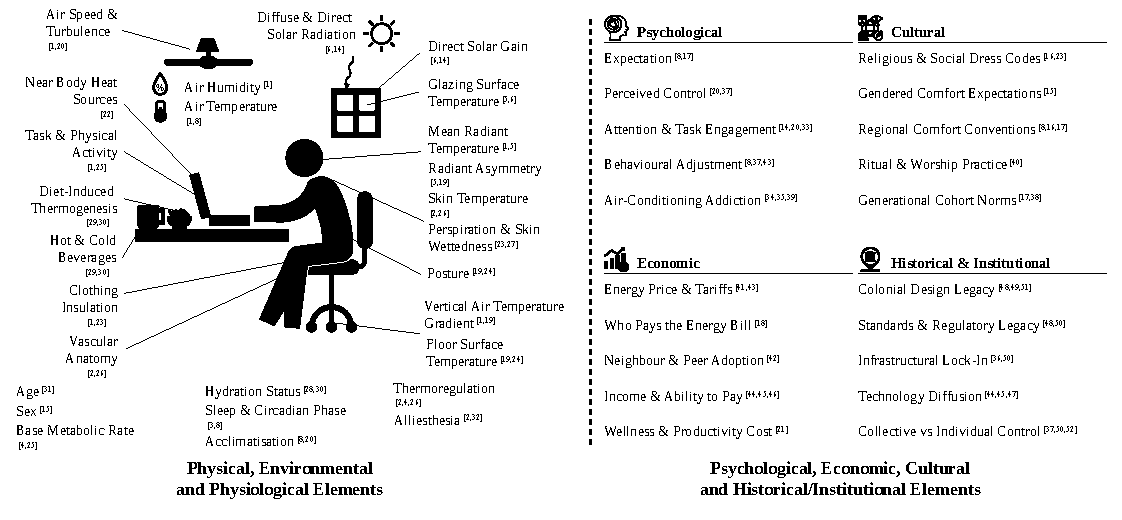
\includegraphics[width=\textwidth]{figures/thermal_preference_elements_v15_190mm_1.pdf}
  \caption{Elements shaping individual thermal preference. The left side groups physical, environmental, and physiological factors around a seated occupant: the surrounding radiant, air-movement, and surface conditions; near-body heat sources, clothing insulation, posture, and physical activity; and physiological state such as skin temperature, perspiration, metabolic rate, hydration, sleep and circadian phase, acclimatization, and thermoregulation. The right side lists psychological, cultural, economic, and historical or institutional factors, ranging from expectation, perceived control, and behavioral adjustment, to dress conventions and regional comfort norms, energy prices and who pays the bill, and colonial design, regulatory, and infrastructural legacies. Together these illustrate why identical ambient conditions can produce heterogeneous thermal-preference responses across individuals.}
  \label{fig:thermal-preference-elements}
\end{figure*}

Characterization of thermal comfort in the built environment has long been dominated by the creation of thermal comfort models, which combine physiology and environmental science to describe when and how a person should feel thermally comfortable or uncomfortable \citep{Fanger1972-xq}.
Rooted in heat-balance theory, these models relate metabolic heat production, clothing insulation, air temperature, radiant conditions, humidity, and air movement to a predicted comfort state, drawing on how core and skin temperatures jointly drive thermal sensation \citep{Frank1999-ju}, how circadian phase and the thermoneutral zone set the body's baseline \citep{Krauchi2002-aq, Kingma2012-lm}, and how radiant and solar exposure adds heat that simple air-temperature metrics miss \citep{Halawa2014-ek, Hodder2007-qo}.
From these inputs, the models predict thermal sensation, satisfaction, and preference, and they remain the backbone of the comfort standards and mechanical systems designed around them \citep{Cheung2019-fs}.
Newer adaptive formulations extend this picture by recognizing that people stay comfortable across a wider range of conditions than heat-balance theory alone would predict, as behavioral adjustment, expectation, and prior thermal history reshape what feels acceptable \citep{Dear1998-va, Schweiker2020-pw}.
Even within the same space, individuals differ systematically in thermal sensitivity and response \citep{Rupp2022-lq, Wang2018-aj}, which is one reason identical ambient conditions can produce the heterogeneous preferences illustrated in Figure~\ref{fig:thermal-preference-elements}.
To capture this variation directly, personal comfort models learn from an individual's own repeated feedback and physiological signals rather than assuming a population average \citep{Arakawa_Martins2022-vh}.
Yet both approaches face practical limits.
Generalized models predict individual thermal sensation correctly only about a third of the time \citep{Cheung2019-fs}, while personal models are difficult to scale because they depend on collecting sustained, labeled data from every occupant \citep{Arakawa_Martins2022-vh}.
Efforts to connect these models to the broader context that surrounds them, including the psychological and non-physical influences that shape perception \citep{Castaldo2018-ih, Chinazzo2019-ye}, demographic and cultural differences in expectation and preference \citep{Karjalainen2012-ag, Naheed2021-ce}, and the social conventions and economics that govern who controls and pays for indoor climate \citep{Shove2003-lf, Gillingham2012-nf}, remain nascent, but they may explain much of why the models still fall short.


\subsection{Thermal behavior varies between people under similar conditions}\label{sec:individual-differences}
% TODO(author): Review adaptive comfort, personal comfort models, expectations,
% alliesthesia, and over-cooling literature.

Given these deficiencies, it is worth looking more closely at the wider set of factors that shape people's thermal experience in cities, which Figure~\ref{fig:thermal-preference-elements} organizes into two broad families.
The left side gathers the physical, environmental, and physiological factors that classical models were built to handle but that continue to surprise us in their detail and interaction.
At the environmental scale, real spaces are rarely uniform, and local asymmetries in radiant, surface, and air-movement conditions shape comfort in ways a single room temperature cannot represent \citep{Su2023-tg}, while personally controlled air movement can restore comfort and even cognitive performance at warmer set points \citep{Schiavon2017-fx, Porras-Salazar2024-mo}.
Closer to the body, near-body heat sources such as laptops \citep{Zhang2014-im}, the insulation and cut of clothing \citep{Havenith2015-yn}, posture \citep{Tikuisis1996-fd}, and physical activity and metabolic rate \citep{Gaesser1975-jn} all shift the balance between heat production and loss.
The physiological state of the occupant adds further variation through cutaneous blood flow \citep{Johnson2010-eh}, sweating and skin wettedness \citep{Fukazawa2009-nx}, hydration \citep{Sawka2001-sz}, the thermic effect of food and drink \citep{Swaminathan1985-ca, Otsuka2021-ty}, and age-related shifts in thermal thresholds \citep{Huang2010-hy}.
Even the pleasantness of a given thermal stimulus depends on internal state, so the same temperature can feel welcome or aversive depending on whether it helps restore the body's balance \citep{Cabanac1971-mg}.
These physical and physiological signals also rarely act alone, combining with the visual, acoustic, and air-quality exposures that any rigorous account of the indoor experience must weigh together \citep{Chinazzo2022-dt}.

The right side of Figure~\ref{fig:thermal-preference-elements} gathers the psychological, cultural, economic, and historical or institutional forces that sit outside the heat balance yet strongly condition how people interpret and act on it.
Psychologically, cooling choices are bound up with identity, values, and the situation at hand rather than temperature alone \citep{Osunmuyiwa2020-fr}, and habitual reliance on air conditioning can harden into a practice that people find difficult to step outside of, even briefly \citep{Hitchings2011-eo}.
Culturally, expectations of what a comfortable indoor climate should feel like are learned and socially organized, shaped by evolving conventions, domestic technology, and the material culture of cooling \citep{Shove2014-fx, Strengers2011-bm, Goodchild2020-ew}, and they take on distinctive forms in specific settings, from the air-conditioned lives of young people in Singapore \citep{Hitchings2008-ky} to the use and energy demand of naturally ventilated places of worship \citep{Atmaca2019-ur}.
Economically, the decision to buy and run cooling responds to weather, prices, incomes, and the efficiency of the available equipment \citep{He2022-rg, Noonan2015-uz, Yun2011-nu}, and as incomes rise and the climate warms, adoption is projected to grow steeply, with large and unequally distributed consequences for electricity demand and emissions \citep{Davis2015-po, Colelli2023-fy, Falchetta2024-ao, Zhang2026-cx}.
Underlying all of this is a historical and institutional legacy in which particular comfort norms, standards, and infrastructures were exported and standardized, homogenizing expectations across very different climates and cultures \citep{Roaf2026-kt, Williamson2025-nt, Healy2008-hk, Winter2013-tm}, a trajectory whose sustainability in an increasingly hot world is now openly in question \citep{Lundgren-Kownacki2018-bv}.

\subsection{Repeated in-situ data can reveal behavioral response patterns}\label{sec:longitudinal-data}
% TODO(author): Position ecological momentary assessment and wearable sensing.

% TODO(author): State the final research questions. A defensible structure is:
% RQ1: Can repeated thermal-preference responses form interpretable person-level
%      behavioural archetypes?
% RQ2: Do archetypes differ in heat dose-response and control-context response?
% RQ3: How robust are the archetypal signatures and memberships?

The convergence of the two major categore
Repeated in-situ reporting provides one route to observing
how thermal preference changes with context and time \cite{Stone1994-he}.

% =============================================================================
\section{Methods}\label{sec:methods}
% =============================================================================


\subsection{Study design, cohort, and data source}\label{sec:data-source}
% TODO(author): Describe the Cozie Singapore smartwatch deployment, ethics,
% consent, time period, response count, participant count, and public
% privacy-protected dataset. Cite the platform and companion dataset paper.
\begin{figure}[htbp]
  \centering
  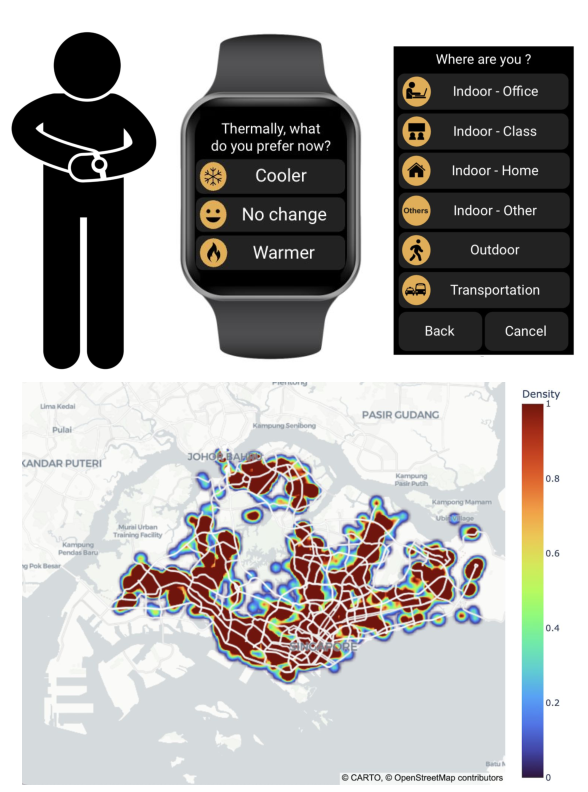
\includegraphics[width=\columnwidth]{figures/cozie_diagram.pdf}
  \caption{Cozie smartwatch micro-survey interface. The thermal-preference question offers Cooler, No change, and Warmer responses; the accompanying location question records the space category at the time of response.}
  \label{fig:cozie-interface}
\end{figure}

\subsection{Survey measures, outdoor heat, and environmental-control context}\label{sec:measures}
% TODO(author): Define thermal preference (Cooler / No change / Warmer), the
% one-hour mean outdoor heat index, location categories, and the a-priori
% contextual grouping by air-conditioning likelihood: Outdoor (No A/C);
% Home (Maybe A/C); Office/Class/Other (Likely A/C); and Transport
% (Very Likely A/C). Explain that outdoor weather is an exposure proxy rather
% than a measurement of individual microclimate.


\subsection{Participant eligibility and person-level features}\label{sec:features}
% TODO(author): Document the all-location eligibility screen (minimum total,
% hot-side, and cool-side observations); empirical-Bayes Beta--Binomial
% shrinkage for P(Cooler) and P(Warmer); and unshrunk within-participant heat
% sensitivity P(Cooler | hot) - P(Cooler | cool). Define the heat split using
% the observed cohort median and give all quantities from executed output.

\begin{figure}[htbp]
  \centering
  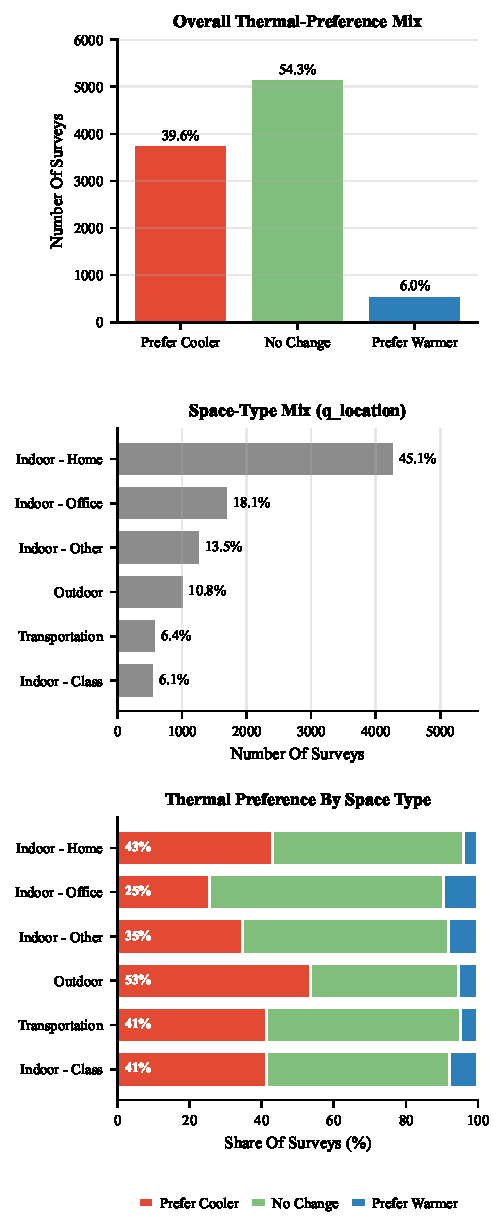
\includegraphics[width=\columnwidth]{figures/00_A2_preference_mix_and_by_space.pdf}
  \caption{Survey composition and thermal preference by space type. Top panel: the overall thermal-preference mix as the number of surveys in each category (Prefer Cooler, No Change, Prefer Warmer), with each category's share of all surveys labeled above its bar. Middle panel: the number of surveys recorded in each space type, with each type's share of all surveys labeled at the end of its bar. Bottom panel: within each space type, the share of surveys indicating Prefer Cooler, No Change, or Prefer Warmer, drawn as a fully stacked bar with the Prefer Cooler share labeled inside each bar.}
  \label{fig:preference-mix-and-by-space}
\end{figure}

\begin{figure*}[t]
  \centering
  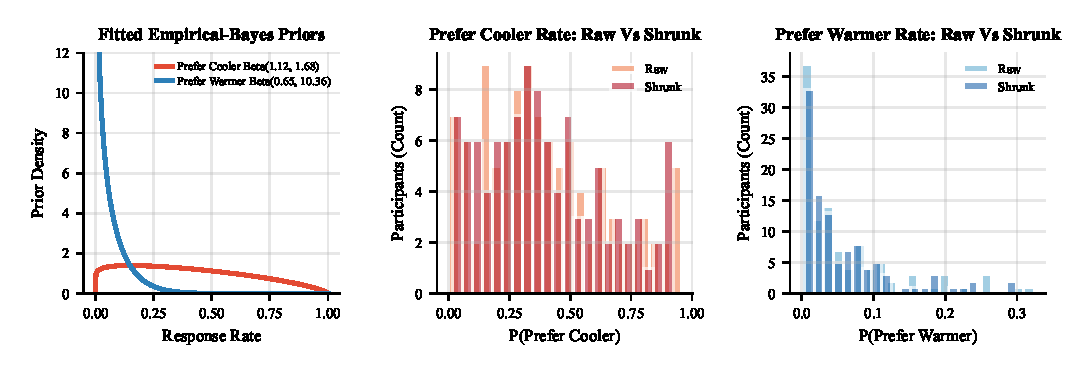
\includegraphics[width=\textwidth]{figures/00_C1_eb_shrinkage.pdf}
  \caption{Empirical-Bayes feature construction. The left panel shows fitted Beta priors for prefer-cooler and prefer-warmer response rates; the center and right panels compare participants' raw and shrunk rates for the two features.}
  \label{fig:eb-shrinkage}
\end{figure*}

\subsection{Archetype discovery and interpretation}\label{sec:clustering}
% TODO(author): Specify standardization, k-means, candidate K range, silhouette
% evaluation, and the explicit interpretability decision to carry K=4 forward.
% Explain transparent post-hoc labels: Unconditional Coolers, Over-Cooled
% Captives, Weather Responders, and Heat-Unbothered. Emphasize that labels are
% descriptive and that membership is expected to be soft at boundaries.

\subsection{Mechanistic scrutiny and robustness checks}\label{sec:scrutiny}
% TODO(author): Pre-specify / describe the following analyses:
% - dose-response of P(Cooler) and P(No change) over outdoor-heat sextiles;
% - P(Warmer) by control context and the Likely-A/C minus Outdoor gradient;
% - heat tolerance versus outdoor exposure;
% - A/C relief across Outdoor and Likely-A/C contexts;
% - participant-cluster bootstrap CIs, seed/subsample stability, alternative
%   heat-threshold agreement, and pairwise Cliff's delta signature contrasts.
% Make clear that survey observations are participant-nested and all inference
% is descriptive/associational rather than causal.

% =============================================================================
\section{Results}\label{sec:results}
% =============================================================================

\subsection{Cohort coverage and thermal-preference context}\label{sec:cohort-results}
% TODO(author): Report executed descriptive results and use a compact initial
% figure/table to establish response coverage, preference mix, space mix, and
% outdoor-heat distribution.

\begin{figure*}[t]
  \centering
  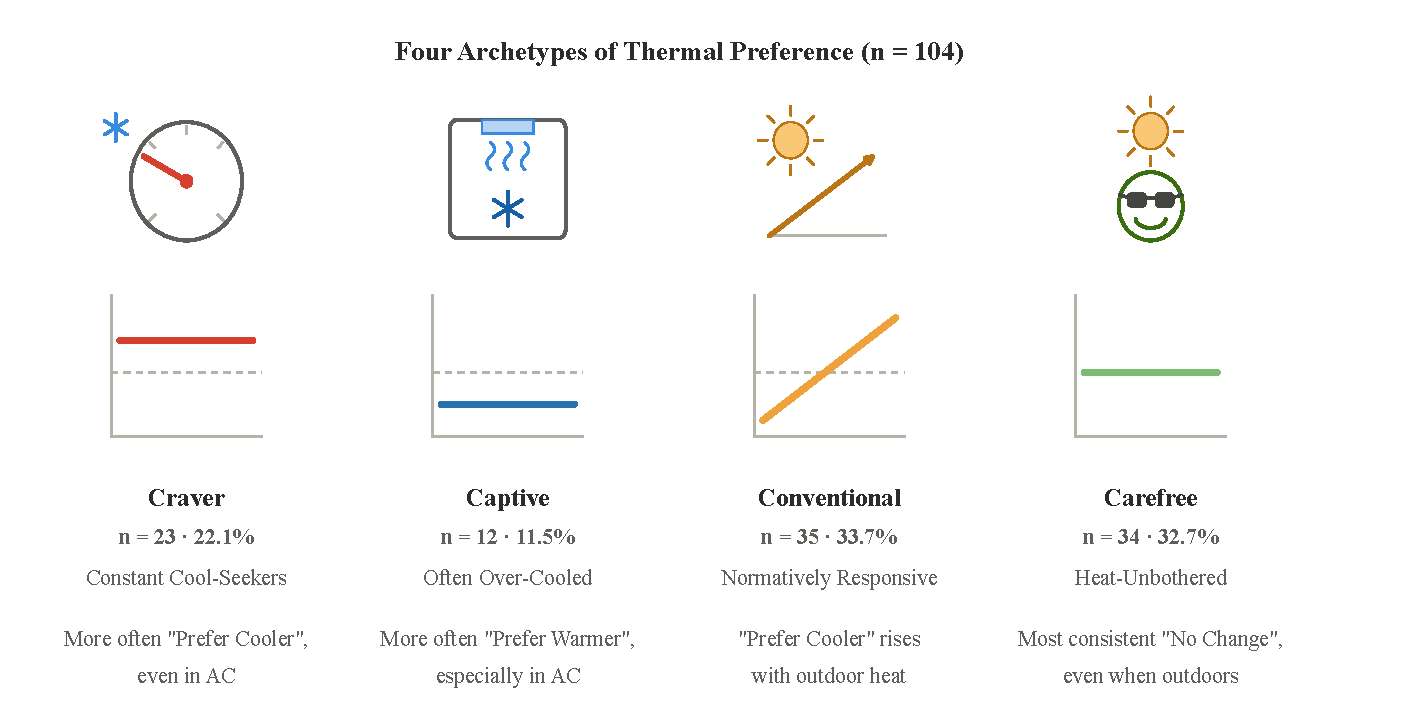
\includegraphics[width=\textwidth]{figures/01_S1_archetype_overview.pdf}
  \caption{Overview of the four behavioral thermal-preference archetypes derived in this study (n = 104 participants). From left to right: the Craver (Constant Cool-Seekers; n = 23, 22.1\%), who prefers cooler more often, even in air-conditioned spaces; the Captive (Often Over-Cooled; n = 12, 11.5\%), who prefers warmer more often, especially in air-conditioned spaces; the Conventional (Normatively Responsive; n = 35, 33.7\%), whose prefer-cooler response rises with outdoor heat; and the Carefree (Heat-Unbothered; n = 34, 32.7\%), who most consistently reports no change, even outdoors. Each column shows a representative icon, a schematic line sketch of the archetype's thermal-preference behavior (axes unlabeled), its name and subtitle, its sample size and share of participants, and a one-line behavioral summary.}
  \label{fig:archetype-overview}
\end{figure*}



\subsection{Behavioral thermal archetypes}\label{sec:archetype-results}
% TODO(author): Present qualification, candidate-K silhouette results, cluster
% separation, group size, and standardized feature signatures. State the small
% K=3 versus K=4 silhouette difference accurately; do not describe K=4 as an
% objectively optimal solution.
\begin{figure*}[t]
  \centering
  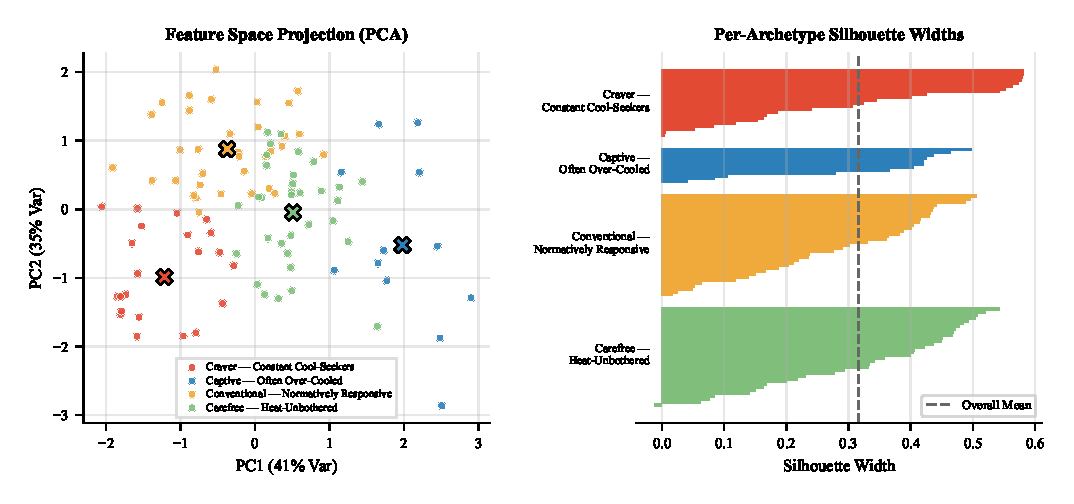
\includegraphics[width=\textwidth]{figures/00_D2_pca_silhouette.pdf}
  \caption{Four-archetype clustering diagnostics. The left panel projects the standardized feature space onto its first two principal components; the right panel shows silhouette widths for individual participants, grouped by archetype.}
  \label{fig:pca-silhouette}
\end{figure*}
\begin{figure}[htbp]
  \centering
  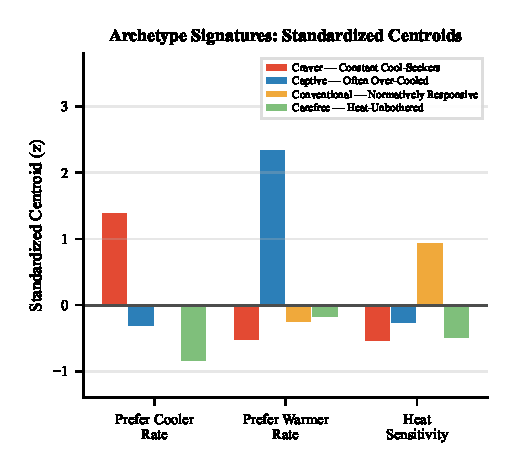
\includegraphics[width=\columnwidth]{figures/00_D3_centroid_profiles.pdf}
  \caption{Standardized feature signatures of the four behavioral thermal archetypes. Lines show cluster centroids for prefer-cooler rate, prefer-warmer rate, and heat sensitivity.}
  \label{fig:centroid-profiles}
\end{figure}

\subsection{Heat dose-response and environmental-control context}\label{sec:mechanistic-results}
% TODO(author): Present the mechanistic scrutiny in a coherent order: heat
% dose-response, over-cooling anatomy, tolerance versus exposure, and A/C
% relief. Give uncertainty and effect sizes from the executed notebook outputs.

\begin{figure*}[t]
  \centering
  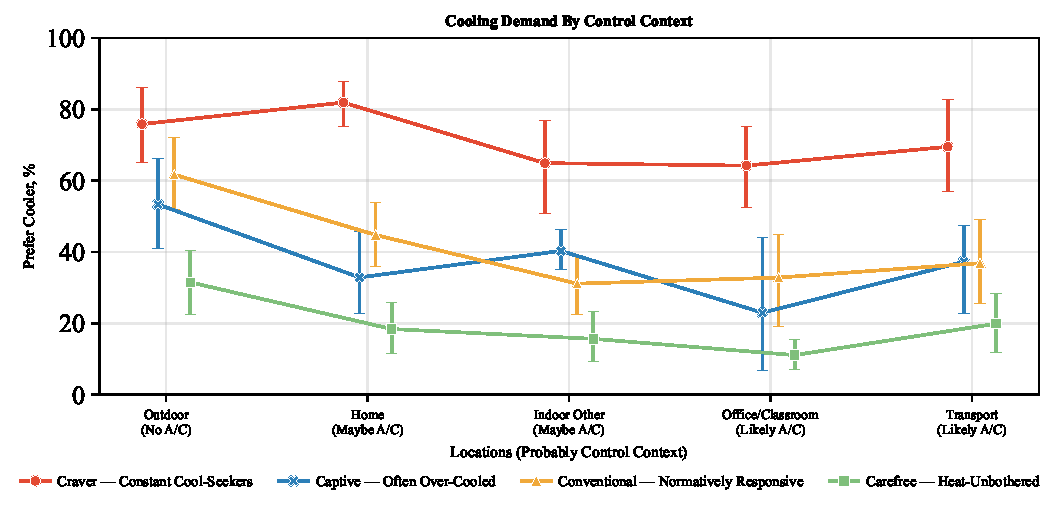
\includegraphics[width=\textwidth]{figures/01_A3_relief_by_context_5cat.pdf}
  \caption{Prefer-cooler responses for each archetype across five probable control contexts, ordered by increasing air-conditioning likelihood (Outdoor with no A/C; Home with maybe A/C; Indoor Other with maybe A/C; Office or Classroom with likely A/C; and Transport with likely A/C), with 95 percent cluster-bootstrap confidence intervals. Each archetype uses a distinct marker in addition to color so the series remain distinguishable in black and white.}
  \label{fig:ac-relief}
\end{figure*}


\begin{figure}[htbp]
  \centering
  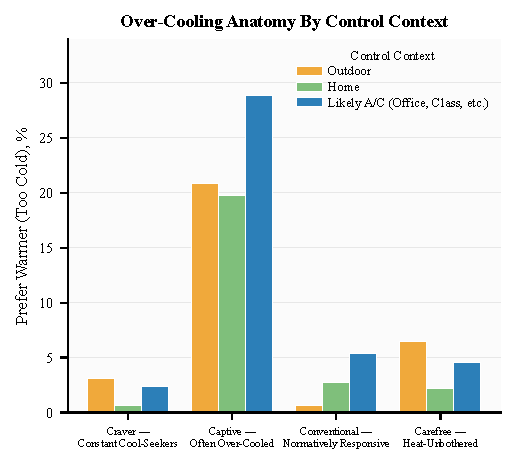
\includegraphics[width=\columnwidth]{figures/01_B1_overcooling_anatomy.pdf}
  \caption{Prefer-warmer (too cold) responses by archetype across the four probable control contexts, ordered by increasing air-conditioning likelihood (Outdoor with no A/C; Home with maybe A/C; Office, Class, or Other indoor with likely A/C; and Transport with very likely A/C). Bars show the percentage of responses indicating a preference for warmer conditions.}
  \label{fig:overcooling-anatomy}
\end{figure}
\begin{figure}[htbp]
  \centering
  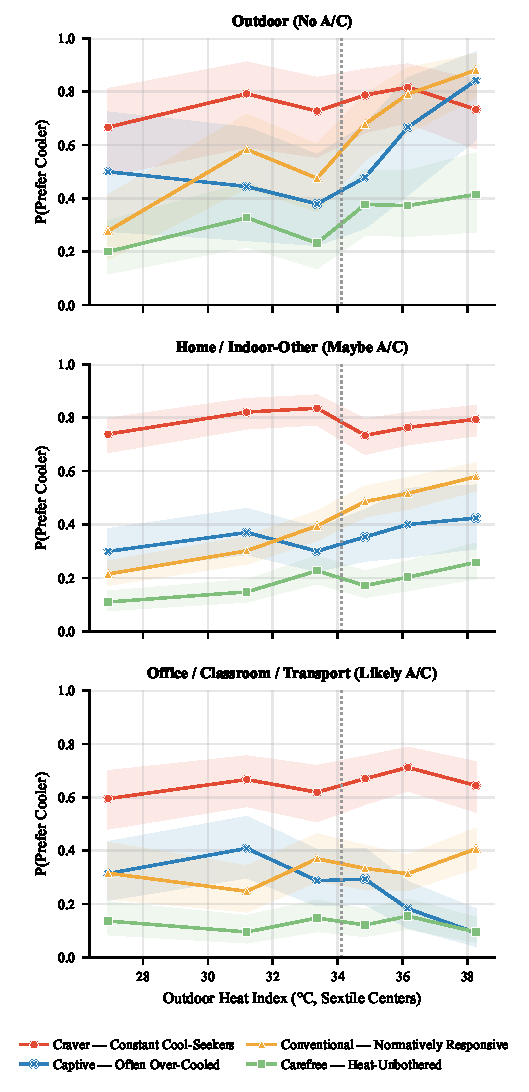
\includegraphics[width=\columnwidth]{figures/01_C3_dose_response_heat_3super.pdf}
  \caption{Probability of preferring cooler conditions versus outdoor heat, shown separately for three probable control supergroups ordered by increasing air-conditioning likelihood (top to bottom: Outdoor with no A/C; Home or Other indoor with maybe A/C; and Office, Classroom, or Transport with likely A/C). Within each panel, one line per archetype gives the prefer-cooler share across outdoor heat-index sextile centers, with Wilson 95 percent intervals as shaded bands and a distinct marker per archetype (Craver, circle; Captive, cross; Conventional, triangle; Carefree, square) so the series remain distinguishable in black and white. The dotted vertical line marks the cohort median heat index.}
  \label{fig:heat-dose-response}
\end{figure}
\begin{figure}[htbp]
  \centering
  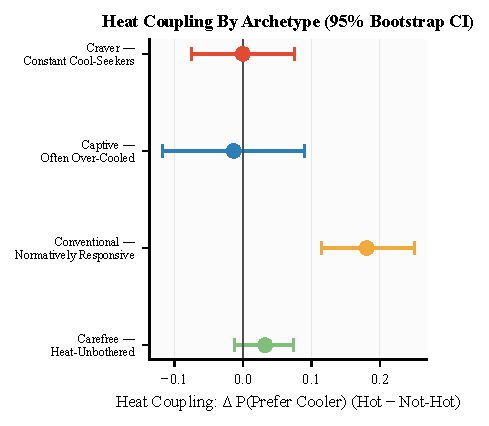
\includegraphics[width=\columnwidth]{figures/01_C2_heat_coupling.pdf}
  \caption{Heat coupling by archetype. Points and horizontal intervals show the difference in participants' prefer-cooler probability between hot and not-hot observations, with 95\% bootstrap confidence intervals.}
  \label{fig:heat-coupling}
\end{figure}
\begin{figure*}[t]
  \centering
  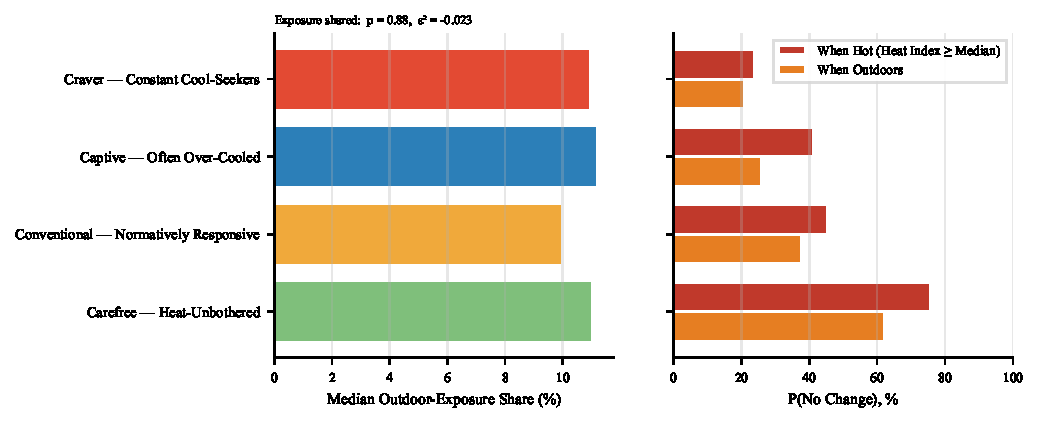
\includegraphics[width=\textwidth]{figures/01_D1_exposure_provoked_comfort.pdf}
  \caption{Outdoor exposure and provoked comfort by archetype. The left panel summarizes participants' outdoor-exposure share; the right panel shows the probability of reporting No Change when observations are both hot and outdoors.}
  \label{fig:exposure-provoked-comfort}
\end{figure*}

\subsection{Robustness and boundary membership}\label{sec:robustness-results}
% TODO(author): Report strong signature separation alongside the observed
% seed/subsample/threshold stability results. Interpret these as support for a
% descriptive continuum discretized into useful archetypes, not a deterministic
% classifier for new individuals.
\begin{figure*}[t]
  \centering
  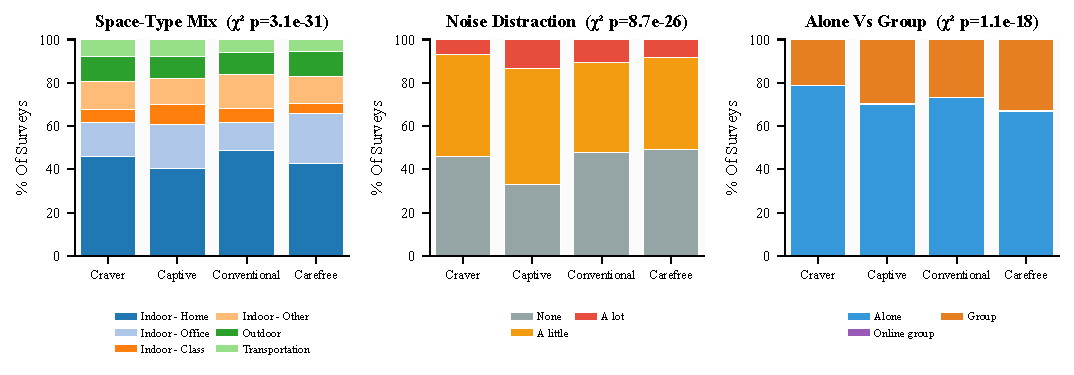
\includegraphics[width=\textwidth]{figures/01_E1_independent_behaviours.pdf}
  \caption{Survey characteristics not used to construct the archetypes. From left to right, panels show the distribution of space type, noise distraction, and alone-versus-group context across the four archetypes.}
  \label{fig:independent-behaviors}
\end{figure*}

% \begin{figure*}[t]
%   \centering
%   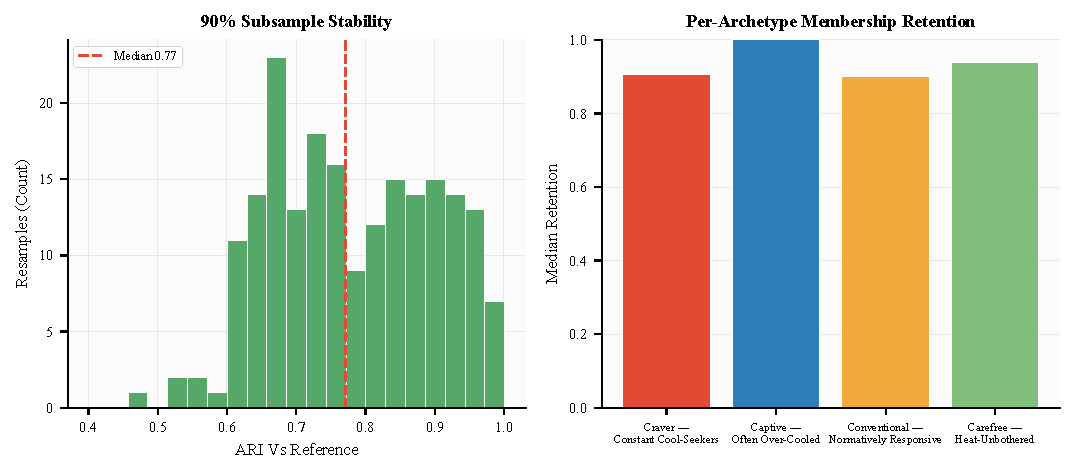
\includegraphics[width=\textwidth]{figures/01_E2_clustering_stability.pdf}
%   \caption{Clustering stability under 90\% participant subsampling. The left panel shows adjusted Rand index values relative to the reference clustering; the right panel shows median archetype-membership retention.}
%   \label{fig:clustering-stability}
% \end{figure*}

\begin{figure*}[t]
  \centering
  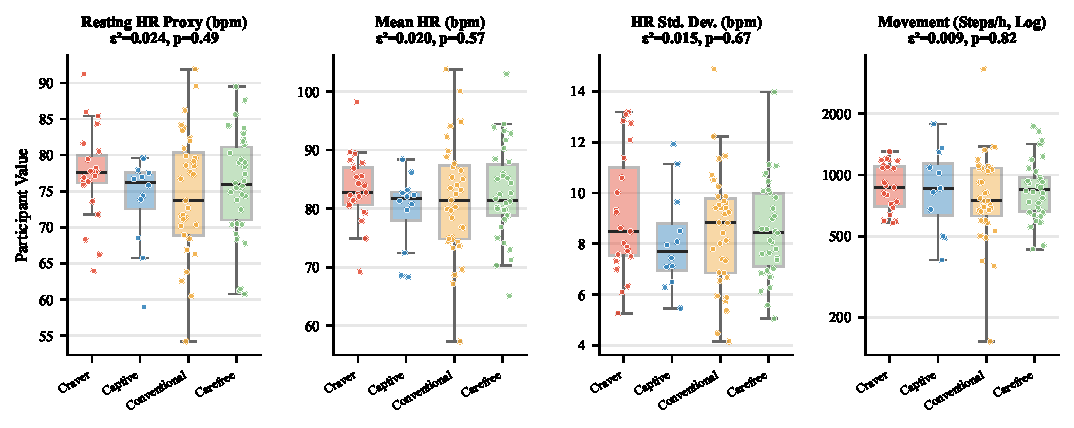
\includegraphics[width=\textwidth]{figures/01_E3_hr_and_movement_by_archetype.pdf}
  \caption{Wearable physiology in the one hour before each survey, summarized to one value per participant and compared across the four archetypes. From left to right: resting heart-rate proxy (mean heart rate on low-activity occasions), mean heart rate, within-hour heart-rate standard deviation (all in beats per minute), and movement (steps per hour, drawn on a logarithmic axis because a single participant is far more active). In each panel the box marks the interquartile range and median and the points are individual participants, colored by archetype. Kruskal-Wallis epsilon-squared effect sizes are all below 0.03 and none of the differences is statistically significant, so the archetypes are not distinguished by heart rate or activity.}
  \label{fig:hr-movement}
\end{figure*}
\begin{figure*}[t]
  \centering
  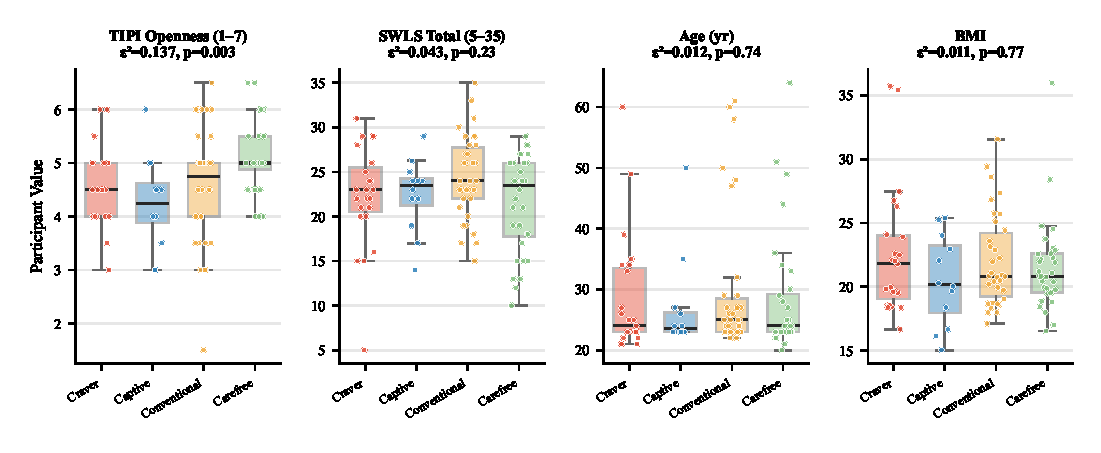
\includegraphics[width=\textwidth]{figures/02_B1_openness_vs_null_dimensions.pdf}
  \caption{Onboarding measures by archetype: one candidate signal against representative null dimensions (n = 101 participants with onboarding data). Each panel shows a participant-level measure across the four archetypes as a box (interquartile range and median) with individual participants overlaid, colored by archetype, and is annotated with the Kruskal-Wallis epsilon-squared effect size and p-value. From left to right: Ten-Item Personality Inventory Openness (1 to 7), Satisfaction With Life Scale total (5 to 35), age in years, and body mass index. Openness is the only measure with a medium effect (epsilon-squared 0.137, p = 0.003), higher in the Carefree type, whereas the other dimensions overlap across archetypes.}
  \label{fig:onboarding-openness}
\end{figure*}

% =============================================================================
\section{Discussion}\label{sec:discussion}
% =============================================================================

\subsection{What the archetypes add to thermal-comfort research}\label{sec:contribution}
% TODO(author): Connect each archetype to the field without reifying the labels
% or assigning traits/causes that were not measured.

\subsection{Implications for buildings, controls, and personalization}\label{sec:implications}
% TODO(author): Discuss design and operation implications at the appropriate
% evidence level. Separate observations about likely A/C contexts from causal
% claims about air-conditioning operation.

\subsection{Strengths and limitations}\label{sec:limitations}
% TODO(author): Address the Singapore cohort, self-selected participants,
% participant-nested observations, weather-as-proxy limitation, location-context
% assumptions, response imbalance, post-hoc cluster naming, and soft membership.

\subsection{Future work}\label{sec:future-work}
% TODO(author): Consider replication in other climates/cohorts, independent
% validation, direct indoor environmental measurements, longitudinal change in
% preferences, and designs that can evaluate causal control interventions.

% =============================================================================
\section{Conclusions}\label{sec:conclusions}
% =============================================================================
% TODO(author): Concisely restate the dataset, typology, verified headline
% patterns, and the calibrated implication for personal thermal comfort and
% built-environment design.

% =============================================================================
\section*{CRediT authorship contribution statement}

% =============================================================================
\section*{CRediT authorship contribution statement}
% =============================================================================
% TODO(author): Replace with the final contributor roles agreed by all authors.
\textit{CRediT roles to be finalized by the authors.}

\section*{Declaration of competing interest}
% TODO(author): Replace with the final journal-compliant declaration.
The authors declare that they have no known competing financial interests or personal relationships that could have appeared to influence the work reported in this paper.

\section*{Acknowledgments}
% TODO(author): Add funders, institutional support, data-collection collaborators,
% and any required grant identifiers after confirming their wording.

\section*{Data availability}
% TODO(author): Replace with the persistent public dataset/repository DOI or URL
% at the point of submission. Do not include private participant information.
The data and analysis materials will be made available in the associated public repository, subject to the privacy protections described in the accompanying data documentation.

\section*{Declaration of generative AI and AI-assisted technologies in the writing process}
% TODO(author): Retain, revise, or remove to match Elsevier's current declaration
% policy at submission and the authors' actual use.
During the preparation of this work, the authors used generative AI tools to assist with organizing and polishing manuscript source files.
The authors reviewed and edited all content and take full responsibility for the final manuscript.

\appendix
\section{Supplementary methods and robustness detail}\label{app:methods}
% TODO(author): Move expanded technical material here only if it supports the
% main text and is not better supplied as separate supplementary material.

\bibliographystyle{elsarticle-num}
\bibliography{cravers-to-carefree}

\end{document}
